\documentclass[12pt]{article}
\usepackage[paper=a4paper,left=30mm,right=30mm,top=35mm,bottom =35mm]{geometry}
\usepackage[utf8]{inputenc}
\usepackage[T1]{fontenc}
\usepackage{stmaryrd}
\usepackage{setspace}
\usepackage{mathrsfs}
\usepackage[ngerman]{babel}
\usepackage{amssymb}
\usepackage{amsmath}
\usepackage{fancyhdr}
\usepackage[dvips,unicode,colorlinks,linkcolor=black]{hyperref} 
\usepackage{graphicx}
\usepackage{float}
\usepackage{listings}

\pagestyle{fancy}
\lfoot{}
\rfoot{Paul Kremser, Tobias Grussenmeyer}
\cfoot{\thepage}
\fancyhead[L]{FPII Versuch: Holographie}
\renewcommand{\headrulewidth}{0.6pt}
\renewcommand{\footrulewidth}{0.6pt}
\setlength{\headheight}{30pt}
\setlength{\parindent}{0pt}
% Für die Wahl der Schriftart
\newcommand{\changefont}[3]{
\fontfamily{#1} \fontseries{#2} \fontshape{#3} \selectfont}
%\renewcommand{\vec}[1]{\mathbf{#1}}
\renewcommand*\vec[1]{{\mbox{\boldmath\ensuremath{#1}}}}

\lstset{
	basicstyle=\ttfamily\scriptsize\mdseries,
	keywordstyle=\bfseries\color{black},
	identifierstyle=,
	commentstyle=\color{black},	
	stringstyle=\itshape\color{black},
	numbers=left,
	numberstyle=\tiny,
	stepnumber=1,
	breaklines=true,
	frame=none,
	showstringspaces=false,
	tabsize=4,
	backgroundcolor=\color{white},
	captionpos=b,
	float=htbp,
	frame=tlrb
%	extendedchars=true
}

\begin{document}
% keine Hurenkinder und Schusterjungen
\clubpenalty = 10000
\widowpenalty = 10000 
\displaywidowpenalty = 10000

\onehalfspacing
% Schriftart
\changefont{ptm}{m}{n} 

\begin{titlepage}
\author{Paul Kremser, Tobias Grussenmeyer}
\title{Versuch: Holographie}
\date{Versuchsdurchführung: 15. bis 19. März 2010} 
\maketitle
\thispagestyle{empty}
\end{titlepage}


\tableofcontents
\thispagestyle{empty}
\newpage
\pagenumbering{arabic}
\section{Überblick}
Holographie ist eine Methode, Objekte dreidimensional abzubilden. Das physikalische Prinzip
der Holographie wurde bereits 1948 von dem Physiker Dennis Gabor entwickelt, der für diese
Erfindung 1971 den Nobelpreis bekam. Er hatte ein
Verfahren entwickelt, mit dem es möglich war, die gesamte Information, also sowohl Amplitude
als auch Phase, eines an einem Objekt gestreuten Wellenfeldes zu speichern.
Während in der Fotografie nur die Amplitude gespeichert wird und man ein zweidimensionales Bild
erhält, gibt eine holographische Aufnahme den vollständigen räumlichen Eindruck wieder. Das Hologramm
wirkt wie ein Fenster, durch das das Objekt betrachtet wird. So ist es
z.B. möglich auch aus einem kleinen Ausschnitt des Hologramms den ganzen Gegenstand zu betrachten,
nur eben aus dem entsprechenden Blickwinkel. Gabors Verfahren besteht
darin, das Objektwellenfeld, das von einem beleuchteten Objekt ausgeht mit einem ungestreuten Wellenfeld, dem Referenzfeld
interferieren zu lassen und das Interferenzmuster auf einer Photoplatte zu speichern. 
Schließlich wird das ursprüngliche Objektfeld mit Hilfe des Referenzfeldes wieder zurück gewonnen (Rekonstruktion). Das Hologramm dient dabei als
Beugungsgitter und die gebeugten Strahlen erzeugen ein Wellenfeld, welches sich vom ursprünglichen Wellenfeld nicht wesentlich unterscheidet.
Eine der wichtigsten Anwendungen der Holographie ist die Interferometrie. Dabei werden auf
einem Film mehrere Hologramme desselben Objekts aufgenommen. Die verschiedenen Bilder
überlagern sich und bilden ein Interferenzmuster, aus dem sich sogar Verformungen im Bereich
der Lichtwellenlänge ermitteln lassen.


\section{Aufgabenstellung}
\begin{itemize}
 \item Mit einem Michelson-Interferometer soll beobachtet werden wie der Optische Aufbau auf Störungen von Außen reagiert und die Kohärenzlänge des Lasers 
      bestimmt werden.
 \item Anfertigung eines Doppelbelichtungshologramms zur Feststellung der Durchbiegung der drei Balken
 \item Untersuchung der Eigenschwingungen der Aluminiumplatte mittels Echtzeitholographie
 \item Beobachtung der Kreuzkorrelation zweier gegeneinander verdrehter Spalte mittels Fourierspektroskopie
\end{itemize}


\section{Theoretische Grundlagen}
\subsection{Licht als elektromagnetische Welle}
Im Prinzip wird jede Funktion die die Wellengleichung
\begin{align}
 \Delta \vec{E} - \frac{1}{v^2} \frac{\partial^2 \vec{E}}{\partial t^2}
\end{align}
löst als Welle bezeichnet. Ein möglicher Ansatz ist der einer harmonischen Welle:
\begin{align}
 \vec{E}(\vec{r},t) = \vec{E_0}(\vec{r}) e^{i(\vec k \vec r \pm \omega t + \delta)}
\end{align}
mit Amplitude $\vec E_0$, Wellenvektor $\vec k$ und Kreisfrequenz $\omega$.
Mit Wellenlänge $\lambda$ und Lichtgeschwindigkeit $c$ gilt außerdem:
\begin{align*}
 c = \frac{\omega}{\left| \vec k \right|} \quad \left|\vec k \right| = \frac{2\pi}{\lambda}
\end{align*}

Wichtige harmonische Wellen sind
\begin{itemize}
 \item Ebene Wellen: Unter einer ebenen Welle im Raum versteht man eine Welle, die zu einem
     bestimmten Zeitpunkt $t$ in allen Ebenen senkrecht zur Ausbreitungsrichtung jeweils eine
     konstante Phase besitzt. Also jede Welle
    \begin{align}
      \vec{E}(\vec{r},t) = \vec{E_0}(\vec{r}) e^{i(\vec k \vec r \pm \omega t)}
    \end{align}
    für die $\vec k\cdot \vec r = const$ gilt.

 \item Kugelwellen: Kugelwellen erhalten ihre große Bedeutung durch das Huygensche Prinzip,
     nach dem jeder von einer Welle erregte Raumpunkt Ausgangspunkt einer neuen Kugelwelle ist.
    Um zu einer Darstellung einer Kugelwelle zu kommen, bei der die Phase auf
     einer Kugelfläche konstant ist, schreibt man die Wellengleichung zweckmäßig in Kugelkoordinaten $(r, \theta, \phi)$
     Mit dem Laplace-Operator in Kugelkoordinaten und der Tatsache, dass Kugelwellen
     sphärisch symmetrisch sind erhält man für die Wellengleichung
    \begin{align}
     \frac{\partial}{\partial r^2} (\vec r \vec E ) - \frac{1}{c^2} \frac{\partial^2}{\partial t^2} (\vec r \vec E) = 0
    \end{align}
    und als Lösung:
    \begin{align}
      \vec{E}(\vec{r},t) = \frac{\vec{E_0}}{\vec{r}} e^{i(\vec k \vec r \pm \omega t)}
    \end{align}
     Die Amplitude $E_0$ fällt proportional zu $\frac{1}{r}$ ab. In großer Entfernung vom Ursprung geht
     die Kugelwelle lokal in eine ebene Welle über.
\end{itemize}

\subsubsection{Interferenz}
Die Linearität der Wellengleichung erlaubt Superpositionen, d.h. jede Linearkombination zweier Lösungen ist wiederum eine Lösung. Die Uberlagerung von Teilwellen bezeichnet man als Interferenz. Überlagert man Wellen mit gleicher Phase, so spricht man von
konstruktiver Interferenz, da diese sich verstärken. Löschen sich die Wellen dagegen gerade gegenseitig
aus, spricht man von destruktiver Interferenz.
Interferieren zwei ebene Wellen gleicher Frequenz $\omega$ und Ausbreitungsrichtung $\vec k$ gilt für die
resultierende Welle folgende Beziehung
\begin{align}
 \vec E_{ges} &= \vec E_1 + \vec E_2 \\
&= \vec E_{01} e^{i(\vec k \vec r + \omega t + \phi_1)} + \vec E_{02} e^{i(\vec k \vec r + \omega t + \phi_2)} \\
&= \left( \vec E_{01} e^{i\phi_1} + \vec E_{02} e^{i\phi_2} \right) e^{i(\vec k \vec r + \omega t)}
\end{align}
Man erhält somit eine neue Welle mit Amplitude $\vec E_{01} e^{i\phi_1} + \vec E_{02} e^{i\phi_2}$. Damit wird die
Intensität $I= \vec E_{0ges}\vec E^*_{0ges}$ zu
\begin{align}
 I &= \vec E^2_{01} + \vec E^2_{02} + \vec E_{01}\vec E_{02} \left( e^{-i(\phi_2 - \phi_1)} + e^{i(\phi_2 - \phi_1)}\right) \\
\label{31} &= I_1 + I_2 + 2\vec E_{01}\vec E_{02} \cos{(\phi_2 - \phi_1)}
\end{align}

Der dritte Summand aus Gleichung \ref{31} wird als Interferenzterm bezeichnet.
Um Interferenzstrukturen beobachten zu können, müssen die Wellen eine feste Phasenbeziehungbesitzen.
Denn falls $\Delta\phi$ beliebige Phasenwinkel zwischen $0$ und $2\pi$ annimmt, mittelt sich der
Interferenzterm aus \ref{31} weg. Strahlt eine Quelle Wellen konstanter Phasenbeziehung ab, so
nennt man sie kohärent. Perfekte Kohärenz gibt es nicht! Es besteht
lediglich die Möglichkeit durch bestimmte experimentelle Anordnungen zeitlich oder räumlich
kohärente Wellen zu erzeugen.
Zeitliche Kohärenz beobachtet der Experimentator, wenn sich die Phasendifferenz während $\delta t$
um weniger als $2\pi$ ändert. Die maximale Zeitspanne $\Delta t$, für die dies gilt, bezeichnet man als
Kohärenzzeit. Eine typische Anordnung zur Erzeugung zeitlich kohärenter Lichtwellen ist der
Laser. Das Produkt aus Kohärenzzeit und Lichtgeschwindigkeit heißt Kohärenzlänge.
Unter räumlicher Kohärenz versteht man, dass sich die Phasendifferenz in einem festen Raumpunkt während der
gesamten Beobachtungszeit um weniger als $2\pi$ ändert. 

Da die Kohärenzlänge einer Lichtquelle angibt, über welche Wegstrecke das Licht eine feste
Phasenbeziehung aufrecht erhalten kann, spielt sie in der Holographie in sofern eine Rolle, als
dass sie dem maximalen Wegunterschied zwischen Referenz- und Objektstrahl entspricht, der
auftreten darf, um noch Interferenzbilder zu erzeugen. Damit ist eine obere Grenze für die Tiefe
des Objekts gegeben, von dem ein Hologramm angefertigt werden kann.

\subsection{Michelson-Interferometer}
Das Michelson-Interferometer ist ein Interferometer, das nach dem Physiker Albert Abraham Michelson benannt wurde. 
Die generelle Funktionsweise eines Interferometers besteht darin, dass eine Lichtwelle in zwei Teile aufzuspalten. Diese zwei Wellen durchlaufen dann
unterschiedlich lange Strecken oder Medien, in denen die Lichtgeschwindigkeit verschieden ist. Dadurch ergibt sich eine Phasenverschiebung zwischen den
zwei Wellen. Werden diese dann wieder zusammengeführt, kommt es zur Interferenz.
\begin{figure}[h]
 \centering
 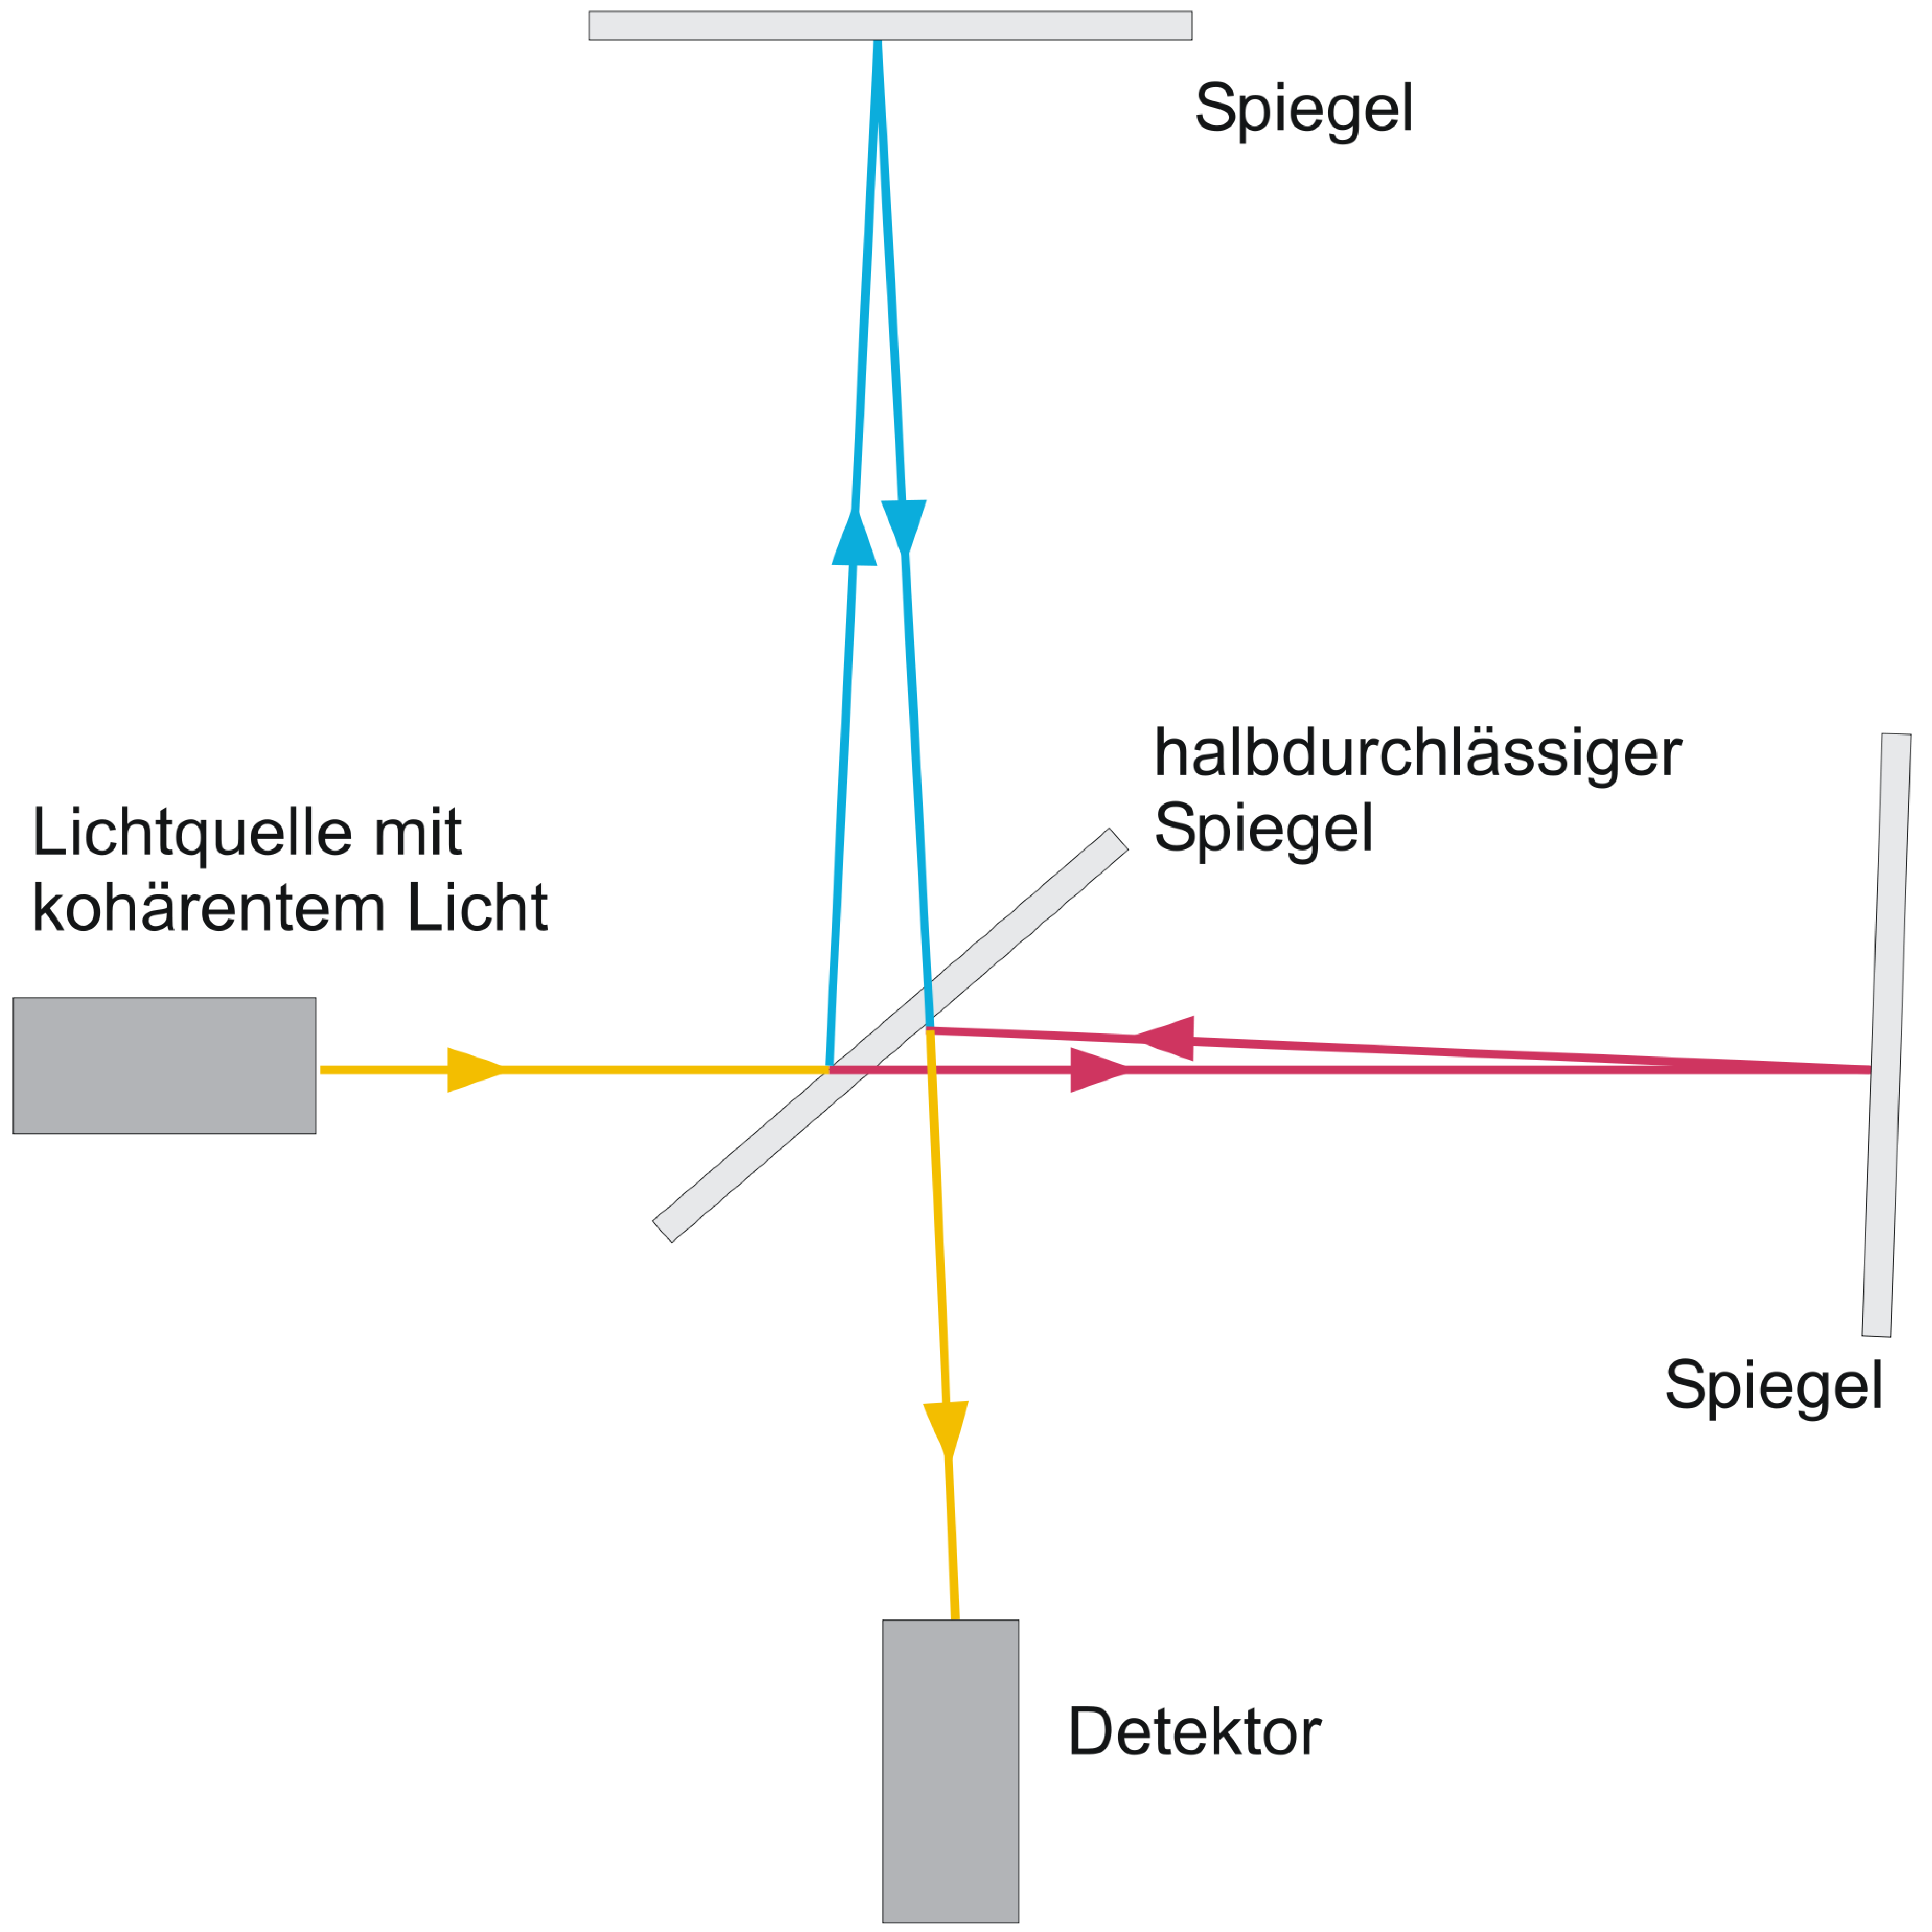
\includegraphics[width=0.5\linewidth]{pictures/michelson.eps}
 \caption{Aufbau Michelson-Interferometer}
 \label{michelson}
\end{figure}
Beim Michelson-Interferometer geschieht die Aufteilung der Lichtwelle mittels eines halbdurchlässigen Spiegels. Siehe Abbildung \ref{michelson}

Verändert man die optische Weglänge einer der beiden Wellen, z.B. indem man einen der beiden Spiegel verschiebt, so verschieben sich die Phasen der beiden
Wellen gegeneinander. Sind sie nun in Phase, so addiert sich ihre Amplitude (man spricht von konstruktiver Interferenz), sind sie jedoch gegenphasig, so
löschen sie sich gegenseitig aus (destruktive Interferenz). Über die Intensitätsmessung der resultierenden Welle können bereits kleinste Veränderungen des
Gangunterschieds zwischen den beiden Wellen gemessen werden.

In unserem Versuch wird das Interferometer dazu verwendet die Kohärenzlänge des Laser zu bestimmen und zu beobachten wie Störungen
(z.B. Schwingungen des Tisches oder der Luft) die Interferenz zerstören.
\subsection{Hologramme}
Auf normalen Fotos ist auf dem Film lediglich Information über die Intensität und bei Farbfotos die Farbe des Lichtes enthalten.

Bei der Holografie wird auf dem Film die Phase und die Intensität gespeichert. Möglich ist dieses durch die Interferenz zweier kohärenter Lichtstrahlen.
Dem sogenannten Referenzstrahl und Objektstrahl. Hierzu wird ein Laser verwedet der durch geeignete Optik aufgefächert wird.
\subsubsection{Aufnahme}
Wird ein beliebiges Objekt mit kohärentem Lich beleuchtet so wird das Licht gebrochen und gestreut. Es entsteht ein Wellenfeld, welches man mit dem Auge
beobachten kann. Dieses Wellenfeld wird Objektwelle genannt. Diese Welle wird mit dem einfallenden ungestreuten Licht (der so genannten Referenzwelle)
überlagert. Das entstehenden Interferenzmuster wird auf einem Lichtempfindlichen Film aufgezeichnet. Die photoempfindliche Schicht des Films reagiert nur auf
die Intensität des Lichtes, durch das Interferenzmuster wird aber die relative Phase (zwischen Objekt- und Referenzwelle) aufgezeichnet.

Voraussetzungen für die Aufzeichnung von Hologrammen ist die zeitliche und räumliche Stabilität der Interferenzmuster. Die aufzuzeichnenden Objekte dürfen
sich während der minutenlangen Belichtung nicht bewegen. Deswegen befindet sich der Aufbau zur Aufnahme des Hologramms auf einem scheren Tisch welcher auf 
einem dämpfenden Material gelagert ist. 

Nach der Entwicklung des Films erhält man ein Gitter, je nach Art des Films bzw. der Entwicklung ist dies ein Amplitudengitter (partikel im Film absorbieren
Teile des Lichts) oder ein Phasengitter (unterschiedliche Brechzahlen im Film), mit dem das Objekt rekonstruiert werden kann.

\subsubsection{Rekonstruktion}
Bei der Rekonstruktion beleuchtet man den Film mit der Referenzwelle. Dabei wird das Licht am Interferenzmuster gebeugt und es entsteht die exakte
Wellenfront der Objektwelle. Hinter dem Hologramm sieht man also den abgebildeten Gegenstand wie durch ein Fenster.
Da auch das ganze Wellenfeld vor und hinter dem aufgezeichneten Objekt rekonstruiert wird, ist man in der Lage das Objekt dreidimensional zu sehen. Dies
wird dadurch weiter verstärkt, dass man sich sogar im Wellenfeld hin- und herbewegen und so den Gegenstand aus verschiedenen Richtungen und, in begrenztem
Ausmaß, auch um ihn herum sehen kann.

Jeder Punkt des abgebildeten Objektes beeinflusst das Wellenmuster des gesamten holografischen Bildträgers. Wenn also ein Hologramm zerteilt wird, kommt bei
der Rekonstruktion noch immer das ganze Bild zustande. Das Aufteilen des Hologramms in einzelne Stücke führt lediglich zu einer Verschlechterung der
Auflösung des Bildes und zu einer Verringerung des ansehbaren räumlichen Bildwinkels.

\subsubsection{Transmissionshologramme}
Transmissionshologramme befinden sich auf lichtdurchlässigen Filmen. Bei der Aufnahme treffen Referenzstrahl und Objektstrahl von der gleichen Seite auf
den Film und erzeugen dort das Interferenzmuster, das aufgenommen wird.
Für die Rekonstruktion des Bildes muss das Transmissionshologramm von hinten mit einer kohärenten Lichtquelle durchleuchtet werden.

\subsubsection{Reflexionshologramme}
Reflexionshologramme reflektieren das einfallende Licht, so dass die Lichtquelle im Gegensatz zu Transmissionshologrammen auf der Seite des Betrachters sein
kann. Bei Reflexionshologrammen treffen Objektstrahl und Referenzstrahl von unterschiedlichen Seiten auf den Film und bilden in ihm das Interferenzmuster, das 
den Film belichtet. Reflexionshologramme sind in jedem Fall Volumenhologramme, d.h. die Dicke des Aufnahmematerials wird zur Speicherung des holografischen 
Bilds genutzt. Es entstehen in dem Film verschiedene Netzebenen, die durch das an den Interferenzmaxima belichteten Stellen des Filmmaterials gehen. Die 
Netzebenen reflektieren bei der Rekonstruktion des Hologramms das einfallende Licht so zurück, dass ein Bild des Gegenstands entsteht. Reflexionshologramme 
sind wegen der Bragg-Bedingung Weißlichthologramme d.h. sie können mit weißem Licht rekonstruiert werden. Hierbei ändert sich die Farbe des virtuellen Bildes
je nach einfallswikel des Lichtes.

\subsection{Doppelbelichtungsholographie}
Bei der Doppelbelichtungsholographie werden zwei verschiedene (räumliche) Zustände des Objekts nacheinander auf einen Film belichtet. Für jeden Zustand wird
dabei die halbe normale Belichtungszeit verwendet. Ist der Unterschied der beiden Zustände nicht zu groß so lässt sich bei der Rekonstruktion eine Überlagerung der
beiden Zustände beobachten. In diesem Versuch werden drei an einem Ende eingespannte Metallbalken durch kleine Gewichte verbogen. Später lassen sich auf dem
virtuellen Bild der Balken Interferenzstreifen beobachten. Aus dem Abstand dieser Streifen kann auf die Stärke der Durchbiegung zurückgeschlossen werden.

Da nur sehr kleine Objektveränderungen betrachtet werden, kann die Intensität der beiden
Aufnahmen als gleich angesehen werden. Für die Amplituden gilt also
\begin{align*}
 \vec E_{01} &= E e^{i\phi_1} \\
 \vec E_{02} &= E e^{i\phi_2}
\end{align*}
und damit ergibt die aus der Überlagerung der beiden Wellen folgende Intensitätsverteilung
\begin{align}
 I = 2E^2(1+\cos{(\phi_2 - \phi_1)})
\end{align}
Die Phasendifferenz $\Delta\phi = \phi_2 - \phi_1$ im Interferenzterm ist eine Funktion der Wegdifferenz des
Lichtes, die durch das Verformen des Objekts entstanden ist. Wird der Objektpunkt $M$ um
die Strecke $D$ senkrecht zur Oberfläche verschoben, so hat dies einen Wegunterschied $d = D(\cos{\alpha} + \cos{\beta})$ zur Folge.
Daraus ergibt sich für die Phasendifferenz
\begin{align}
 \Delta\phi = \frac{2\pi}{\lambda} D(\cos{\alpha} + \cos{\beta})
\end{align}
% und damit unter Anwendung von Additionstheoremen für die Intensität
% \begin{align}
%  I = 4E^2 \cos{\frac{2\pi}{\lambda}} D(\cos{\alpha} + \cos{\beta})^2
% \end{align}
% Die Intensität ändert sich also mit $\cos^2$ , wobei das Argument bis auf einen konstanten Faktor,
% nämlich die Verschiebung D, bestimmt ist. Zwei Interferenzstreifen entstehen also durch Verschiebung um
% \begin{align}
%  D =\frac{\lambda}{\cos{\alpha} + \cos{\beta}}
% \end{align}
???



Die Durchbiegungskurven haben die Form:
\begin{align}
 y = P_1 \left(5 x^2 - \frac{x^3}{6}\right) + P_2 x + P_3
\end{align}
wobei $x$ der Abstand von der Einspannstelle, $y$ die Auslenkung aus der Ruhelage und $P_{1,2,3}$ Material bzw. Aufbaubedingt sind.

\section{Durchführung}
\subsection{Michelson-Interferometer}
Zu Anfang des Versuchs haben wir das Michelson-Interferometer aufgebaut. Hierzu verwendeten wir den Strahlteiler, zwei Spiegel und einen Schirm. Siehe
Abbildung %\ref{michelson-photo}
Angefangen mit gleicher Weglänge für beide Teilstrahlen, beobachteten wir den Einfluss von Schwingungen auf das Interferenzbild durch Klopfen auf den Tisch,
lautes Sprechen, Stampfen auf dem Boden und Entzündung einer Flamme unter einem Teilstrahl. Schließlich vergrößerten wir einen der beiden Wege bis kein 
Interferenzmuster mehr zustande kam. Bevor das Bild ganz verschwindet, kann man ein Wandern oder ``Athmen'' im Bild beobachten.

\subsection{Holografie}
\subsubsection{Justierung der Optik}
Nachdem wir festgestellt hatten, dass die Strahlteilerscheibe wohl einen ``achter'' hat und somit den reflektierten Strahl bei Änderung der Intensität leicht
verschiebt, entschieden wir diesen für die Objektwelle zu verwenden. Damit war es uns möglich zuerst Raumfilter und Spiegel des Referenzstrahls bei maximaler
Intensität zu justieren und anschließend das für die Aufnahme verwendete Intensitätsverhältnis (wesentlich mehr Intensität für Objektwelle) einzustellen. Nun 
konnten auch Raumfilter und Spiegel des Objektstrahls justiert werden, ohne danach nochmals an dem Strahlteiler drehen zu müssen.
Wie wir schon vorher erfahren hatten, benötigt das Justieren der Raumfilter einige Übung. Das Vorgehen besteht im Wesentlichen darin, das Objektiv
ohne Pinnhole im Strahlengang so zu positioniern, dass der Strahl mittig durchläuft und nicht abgelenkt wird. Dies lässt sich ziemlich gut erreichen
indem
man die Reflexion des Strahls an der Linse betrachtet: Man lässt den Strahl auf dem Weg zum Objektiv durch ein gelochtes Stück Papier laufen, bilden die 
Reflexionen am Objektiv auf diesem Papier konzentrische Kreise um das Loch, ist das Objektiv perfekt positioniert.
Danach wird das Pinnhole auf den Schlitten aufgesetzt
und bis auf ca. $1mm$ an das Objektiv herangeschoben und dort fixiert. Nun versucht man Grob das Pinnhole mit den beiden Senkrecht zu Strahl stehenden Achsen
so zu Positionieren, dass der Strahl mittig auf die Folie trifft. Bringt man nun das Pinnhole noch etwas näher an das Objektiv und variiert danach wieder die
beiden senkrechten Achsen, so kann man einen sehr intensitätsschwachen verschwommenen Lichtpunkt auf dem Schirm finden. Schließlich gilt es das Pinnhole immer
näher an das Objektiv zu bringen und dabei immer wieder den Lichtkegel mit den beiden senkrechten Achsen auf die ursprüngliche Position zu verschieben, bis 
ein Bereich etwa der Größe des Spiegels vollständig gleichmäßig beleuchtet ist.

Nach dem Einstellen der beiden Raumfilter, werden Spiegel , Objekt und Filmhalterung positioniert. Hierbei ist die Kohärenzlänge des Lasers zu beachten.
Leider ist die vorhandene Kombination aus Magnetfuß, Spiegel und Stange nicht auf den restlichen Aufbau abgestimmt. Die Spiegel lassen sich somit nicht tief
genug positionieren um den Aufgespalteten Strahl optimal auszunutzen. Außerdem sind die Magnetfüße teilweise so schlecht, dass man sich gar nicht sicher ist
ist welche Einstellung (Magnet senkrecht / waagerecht) besseren halt bietet. So kam es oft vor, dass die komplette Justierung wiederholt werden musste, da man
aus Versehen irgentwo drangekommen war.

\subsubsection{Belichtung und Entwicklung}
Da die am Versuch vorhandene Photodiode defekt was, gab es keine Möglichkeit die Intensität am Ort des Films zu messen. Somit konnten wir die Belichtungszeit
nicht ausrechenen sonder nur ausprobieren. Wir versuchten Werte von $10s$, $3min$, $5min$, $10min$ und $12min$. Bei allen Zeiten war nach dem Entwickeln eine
Schwärzung des Films zu sehen. Bei Zeiten unter $5min$ war jedoch schon nach kurzer Zeit im Bleichbad absolut nichts mehr auf dem Film zu sehen. Bei größeren
Zeiten, war nach ca. $2min$ bleichen die Schwärzung verschwunden und gelbliche Ringartige Strukturen zu erkennen. Wir entschieden uns Schließlich für:
$12min$ Belichten, $1min$ Entwickeln $2min$ Bleichen und ca $20min$ Wässern.

\subsubsection{Rekonstruktion}
Nachdem wir die Balken jeweils $6min$ mit und $6min$ ohne angehängte Gewichte belichtet, entwickelt, gebleicht, gewässert und getrocknet hatten, plazierten
wir das Hologramm wieder zwischen den beiden Glasscheiben und entfernten das Objekt. Mit der Videokamera am Versuch war es zwar möglich das Hologramm zu sehen,
jedoch nicht ein Bild der Messskala (Rechter Winkel) und des Hologramms gleichzeitig aufzunehmen. Mit Hilfe einer digitalen Spiegelreflexkamera konnten wir
solch Bilder anfertigen. Hierzu haben wir die Skala während der Belichtung kurz mit einer Taschenlampe beleuchtet. Wie man an den Bildern sieht, ist es uns
nicht gelungen ein Hologramm anzufertigen das an allen Punkten die Information trägt. Es gab immer Stellen im Hologramm an denen man das Objekt nicht sehen 
konnte. Aus den Fotos konnten wir ziemlich gut die Position der Minima auf den Balken bestimmen.

\subsection{Weiteres}
Da der Aufbau des öfteren, insbesondere jeden Morgen eigentlich kommplett neu durchgeführt werden musste kamen wir erst am letzten Tag zur Echtzeitholographie
leider haben wir es nicht mehr geschafft in der Verbleibenden Zeit ein funktionierendes Hologramm der Aluplatte anzufertigen.

\section{Auswertung}
\begin{figure}[h]
\centering
 \includegraphics[width=0.5\linewidth]{pictures/staebe.eps}
 \caption{Aufbau Michelson-Interferometer}
\end{figure}

\begin{figure}[h]
\centering
 \includegraphics[width=0.5\linewidth]{pictures/staebe-skala.eps}
 \caption{Aufbau Michelson-Interferometer}
\end{figure}
\section{Zusammenfassung}

\section{Anhang}

\subsection{Quelltext}

\lstinputlisting[language=python, extendedchars=false, inputencoding=utf8]{../staebe/staebe.py}

\end{document}
